\documentclass[10pt]{article}

\usepackage[a4paper,margin=0.2in]{geometry}
\usepackage{fontspec}
\usepackage{listings}
\usepackage{color}
\usepackage[framemethod=TikZ]{mdframed}
\usepackage[parfill]{parskip}
\usepackage{hyperref}
\usepackage{graphicx}

\setmainfont{Fira Sans}
\setmonofont{Fira Mono}
\newfontface\BoldMonoFont{Fira Mono Bold}[]

\pagenumbering{gobble}

\definecolor{gray}{RGB}{34, 34, 34}
\definecolor{red}{RGB}{248, 103, 78}
\definecolor{carminepink}{rgb}{0.92, 0.3, 0.26}
\definecolor{darkelectricblue}{rgb}{0.33, 0.41, 0.47}
\definecolor{antiquewhite}{rgb}{0.98, 0.92, 0.84}
\definecolor{columbiablue}{rgb}{0.61, 0.87, 1.0}
\definecolor{cadmiumgreen}{rgb}{0.0, 0.42, 0.24}
\definecolor{cobalt}{rgb}{0.0, 0.28, 0.67}
\definecolor{darkorange}{rgb}{1.0, 0.55, 0.0}
\definecolor{grannysmithapple}{rgb}{0.66, 0.89, 0.63}
\definecolor{atomictangerine}{rgb}{1.0, 0.6, 0.4}

\hypersetup{unicode=true,
            colorlinks=true,
            urlcolor=cobalt,
            breaklinks=true}

\lstset{
    inputencoding=utf8,
    extendedchars=true,
    aboveskip=0.5em,
    backgroundcolor=\color{white},
    basicstyle=\normalsize\ttfamily\color{black},
    breakatwhitespace=false,
    breaklines=true,
    captionpos=b,
    escapeinside={\%*}{*)},
    keywordstyle=\BoldMonoFont\color{carminepink},
    identifierstyle=\color{black},
    stringstyle=\color{cadmiumgreen},
    commentstyle=\color{darkelectricblue},
    showspaces=false,
    showstringspaces=false,
    showtabs=false,
    stepnumber=2,
}

\mdfsetup{
    nobreak=true,
    outerlinewidth=0,
    innerlinewidth=0,
    outerlinecolor=red!90,
    innerlinecolor=red!90,
    roundcorner=4pt,
    leftmargin=3,
    rightmargin=3,
    backgroundcolor=white,
    innertopmargin=0,
    innerbottommargin=10,
    innerleftmargin=9,
    innerrightmargin=9,
    splittopskip=\topskip,
}


\pagecolor{columbiablue!50}

\begin{document}

\twocolumn[
    \begin{@twocolumnfalse}
        \begin{mdframed}
            \begin{minipage}{21.7em}
                \vspace{1.0em}
                {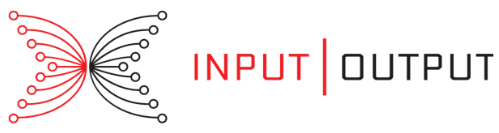
\includegraphics[scale=0.7]{tex/img/iohk-logo.png}}
            \end{minipage}
            \begin{minipage}{28.8em}
                \vspace{0.95em}
                \Large{BENCHMARKING}
            \end{minipage}
            \begin{minipage}{2.5em}
                \vspace{1.0em}
                \href{https://github.com/input-output-hk/iohk-monitoring-framework}{GitHub}
            \end{minipage}
        \end{mdframed}
        \vspace{0.75em}
    \end{@twocolumnfalse}
]

\begin{mdframed}
    \section*{\href{https://github.com/input-output-hk/iohk-monitoring-framework/blob/master/iohk-monitoring/src/Cardano/BM/Observer/Monadic.lhs}{Benchmarking on monad evaluation}}

The bracket around an IO action will enter a named context, evaluate the action, and return its result. A bracket, in a named context, can be placed around a STM action:

    \begin{lstlisting}[language=Haskell]
bracketObserveIO
    :: Configuration
    -> Trace IO a
    -> Severity
    -> Text
    -> IO t
    -> IO t
    \end{lstlisting}

The set of observed counters are traced as \texttt{ObserveOpen}, \texttt{ObserveClose} and \texttt{ObserveDiff} with the indicated severity to the Trace. An exception thrown in the action will be traced and rethrown.

Other bracketing functions exist: \texttt{bracketObserveM} and \texttt{bracketObserveX}.
\end{mdframed}

\begin{mdframed}

    \section*{\href{https://github.com/input-output-hk/iohk-monitoring-framework/blob/master/iohk-monitoring/src/Cardano/BM/Observer/STM.lhs}{Benchmarking STM transaction}}

A bracket, in a named context, can be placed around an STM action:

    \begin{lstlisting}[language=Haskell]
bracketObserveIO
    :: Configuration
    -> Trace IO a
    -> Severity
    -> Text
    -> STM t
    -> IO t
    \end{lstlisting}

This will return the result from successfully evaluating the STM action, which does not have access to logging.

A second bracket function also traces the log items (pairs of meta data and content) which are output by the STM action and returns its result.

    \begin{lstlisting}[language=Haskell]
bracketObserveLogIO
    :: Configuration
    -> Trace IO a
    -> Severity
    -> Text
    -> STM (t,[(LOMeta, LOContent a)])
    -> IO t
    \end{lstlisting}
\end{mdframed}

\begin{mdframed}

    \section*{\href{https://github.com/input-output-hk/iohk-monitoring-framework/blob/master/iohk-monitoring/src/Cardano/BM/Data/Aggregated.lhs}{Aggregation}}

Observables can be forwarded for aggregation, which currently can aggregate them into a basic statistics or an exponentially weighted moving average (EWMA).

Aggregated values reenter the switchboard with '\#aggregation' prepended to their name, and can be routed like ordinary messages.

Values may be of type:

    \begin{lstlisting}[language=Haskell]
data Measurable
    = Microseconds
    | Nanoseconds
    | Seconds
    | Bytes
    | Severity
    | PureI Integer
    | PureD Double
    \end{lstlisting}

The statistics computes: minimum, maximum, mean, std. dev., and count of (1) the observed values, (2) their differences to the previous, and (3) the time between messages.
\end{mdframed}

\begin{mdframed}

    \section*{\href{https://github.com/input-output-hk/iohk-monitoring-framework/blob/master/iohk-monitoring/src/Cardano/BM/Data/Counter.lhs}{Observables --- OS counters}}

Platform independent:

\texttt{MonotonicClock }clock with μs precision\newline
\texttt{GhcRtsStats    }Haskell RTS values (gc, mem)

Linux specific:

\texttt{MemoryStats    }reports memory usage\newline
\texttt{ProcessStats   }lots of process info: cpu, mem, io, ...\newline
\texttt{IOStats        }block device I/O\newline
\texttt{NetStats       }network I/O

The Linux specific counters for the current process are obtained from the \texttt{/proc} interface into the kernel.

To trace observables, the configuration needs to find a definition of a subtrace ObservableTrace for the context name. Only the mentioned counters in the list will be recorded.

    \begin{lstlisting}[language=Haskell]
CM.setSubTrace
    config
    "proc.observed"
    (Just $ ObservableTrace observablesSet)
  where
    observablesSet = [ MonotonicClock
                     , MemoryStats
                     ]
    \end{lstlisting}

%    A complete example of bracketing monadic and STM actions is in \texttt{example-complex}. Run it with:
%
%    \begin{lstlisting}[language=Bash]
%cabal new-run example-complex
%    \end{lstlisting}
%
%or
%
%    \begin{lstlisting}[language=Bash]
%stack run example-complex
%    \end{lstlisting}
\end{mdframed}

\end{document}
